\begin{figure}
    \centering
    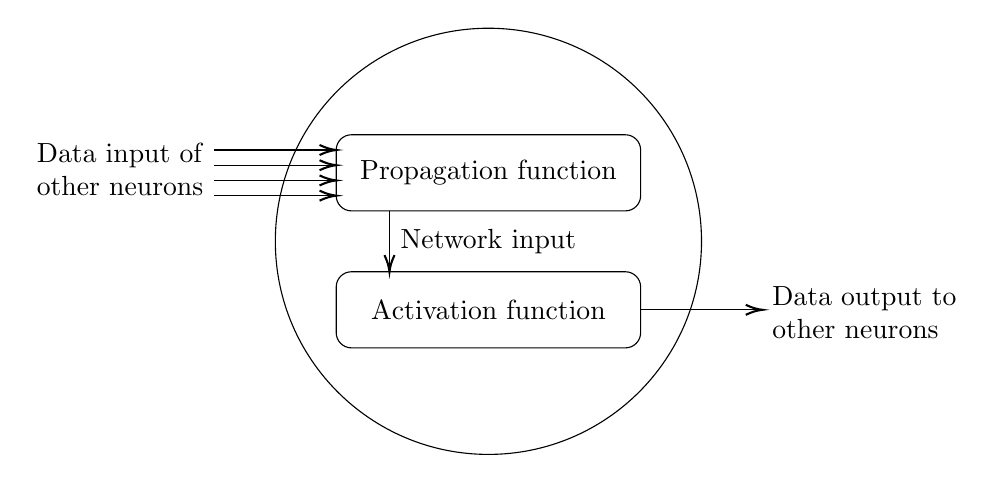
\begin{tikzpicture}[x=0.55pt,y=0.55pt,yscale=-1,xscale=1]
        %uncomment if require: \path (0,300); %set diagram left start at 0, and has height of 300
        
        %Shape: Circle [id:dp16703115491619047] 
        \draw   (155,150) .. controls (155,72.68) and (217.68,10) .. (295,10) .. controls (372.32,10) and (435,72.68) .. (435,150) .. controls (435,227.32) and (372.32,290) .. (295,290) .. controls (217.68,290) and (155,227.32) .. (155,150) -- cycle ;
        %Rounded Rect [id:dp968097124870297] 
        \draw   (195,90) .. controls (195,84.48) and (199.48,80) .. (205,80) -- (385,80) .. controls (390.52,80) and (395,84.48) .. (395,90) -- (395,120) .. controls (395,125.52) and (390.52,130) .. (385,130) -- (205,130) .. controls (199.48,130) and (195,125.52) .. (195,120) -- cycle ;
        %Rounded Rect [id:dp48825970598888957] 
        \draw   (195,180) .. controls (195,174.48) and (199.48,170) .. (205,170) -- (385,170) .. controls (390.52,170) and (395,174.48) .. (395,180) -- (395,210) .. controls (395,215.52) and (390.52,220) .. (385,220) -- (205,220) .. controls (199.48,220) and (195,215.52) .. (195,210) -- cycle ;
        %Straight Lines [id:da28699213799346746] 
        \draw    (230,130) -- (230,168) ;
        \draw [shift={(230,170)}, rotate = 270] [color={rgb, 255:red, 0; green, 0; blue, 0 }  ][line width=0.75]    (10.93,-3.29) .. controls (6.95,-1.4) and (3.31,-0.3) .. (0,0) .. controls (3.31,0.3) and (6.95,1.4) .. (10.93,3.29)   ;
        
        %Straight Lines [id:da4660434658597914] 
        \draw    (115,90) -- (193,90) ;
        \draw [shift={(195,90)}, rotate = 180] [color={rgb, 255:red, 0; green, 0; blue, 0 }  ][line width=0.75]    (10.93,-3.29) .. controls (6.95,-1.4) and (3.31,-0.3) .. (0,0) .. controls (3.31,0.3) and (6.95,1.4) .. (10.93,3.29)   ;
        
        %Straight Lines [id:da9228038405838919] 
        \draw    (115,100) -- (193,100) ;
        \draw [shift={(195,100)}, rotate = 180] [color={rgb, 255:red, 0; green, 0; blue, 0 }  ][line width=0.75]    (10.93,-3.29) .. controls (6.95,-1.4) and (3.31,-0.3) .. (0,0) .. controls (3.31,0.3) and (6.95,1.4) .. (10.93,3.29)   ;
        
        %Straight Lines [id:da7128529944980109] 
        \draw    (115,110) -- (193,110) ;
        \draw [shift={(195,110)}, rotate = 180] [color={rgb, 255:red, 0; green, 0; blue, 0 }  ][line width=0.75]    (10.93,-3.29) .. controls (6.95,-1.4) and (3.31,-0.3) .. (0,0) .. controls (3.31,0.3) and (6.95,1.4) .. (10.93,3.29)   ;
        
        %Straight Lines [id:da21112944427932812] 
        \draw    (115,120) -- (193,120) ;
        \draw [shift={(195,120)}, rotate = 180] [color={rgb, 255:red, 0; green, 0; blue, 0 }  ][line width=0.75]    (10.93,-3.29) .. controls (6.95,-1.4) and (3.31,-0.3) .. (0,0) .. controls (3.31,0.3) and (6.95,1.4) .. (10.93,3.29)   ;
        
        %Straight Lines [id:da7928692563036984] 
        \draw    (395,195) -- (473,195) ;
        \draw [shift={(475,195)}, rotate = 180] [color={rgb, 255:red, 0; green, 0; blue, 0 }  ][line width=0.75]    (10.93,-3.29) .. controls (6.95,-1.4) and (3.31,-0.3) .. (0,0) .. controls (3.31,0.3) and (6.95,1.4) .. (10.93,3.29)   ;
        
        
        % Text Node
        \draw (53,103) node  [align=left] {Data input of\\other neurons};
        % Text Node
        \draw (295,105) node  [align=left] {Propagation function};
        % Text Node
        \draw (295,195) node  [align=left] {Activation function};
        % Text Node
        \draw (295,150) node  [align=left] {Network input};
        % Text Node
        \draw (542,197) node  [align=left] {Data output to\\other neurons};
    \end{tikzpicture}
    \caption{Data processing of a neuron.}
    \label{neuron_data_processing}
\end{figure}